\documentclass[aspectratio=169,10pt,compress]{beamer}

\useoutertheme{split}
\useinnertheme{rounded}
\usecolortheme{whale}
\usecolortheme{orchid}
\setbeamertemplate{blocks}[rounded]
\setbeamertemplate{navigation symbols}{}
\setbeamertemplate{page number in head/foot}[totalframenumber]
% split footline shows "i / N" (frame number / total frames) on every frame

\usepackage[T1]{fontenc}
\usepackage{lmodern}
\usepackage{listings}
\usepackage{xcolor}
\usepackage{booktabs}
\usepackage{array}
\usepackage{tikz}
\usetikzlibrary{positioning,arrows.meta,calc,matrix}

\newcolumntype{L}[1]{>{\raggedright\arraybackslash}p{#1}}

\definecolor{codebg}{RGB}{245,245,245}
\definecolor{codecomment}{RGB}{110,110,110}
\definecolor{gitred}{RGB}{240,80,50}
\definecolor{gitblue}{RGB}{40,90,160}
\definecolor{gitgreen}{RGB}{40,130,70}

\lstset{
  language=bash,
  basicstyle=\ttfamily\footnotesize,
  backgroundcolor=\color{codebg},
  commentstyle=\color{codecomment}\itshape,
  keywordstyle=\color{gitred}\bfseries,
  morekeywords={git},
  frame=single,
  rulecolor=\color{gray!40},
  columns=fullflexible,
  keepspaces=true,
  showstringspaces=false,
  breaklines=true,
  xleftmargin=4pt,
  xrightmargin=4pt,
  aboveskip=4pt,
  belowskip=4pt
}

\newcommand{\cmd}[1]{\texttt{\color{gitred}#1}}

\tikzset{
  commit/.style={circle, draw=gitblue, fill=gitblue!15, thick, minimum size=7mm,
                 inner sep=0pt, font=\scriptsize\ttfamily},
  newcommit/.style={commit, draw=gitred, fill=gitred!15},
  edge/.style={-{Stealth[length=2mm]}, thick, gray!70},
  lbl/.style={font=\scriptsize\bfseries, text=gitred},
  ref/.style={draw=gitred, thick, fill=gitred!12, rounded corners=2pt,
              font=\scriptsize\ttfamily, inner sep=2pt},
  headref/.style={ref, draw=gitblue, fill=gitblue!12},
  ptr/.style={-{Stealth[length=1.6mm]}, thick, gitred}
}

\definecolor{oldred}{RGB}{200,30,30}
\definecolor{newblue}{RGB}{25,75,200}
\definecolor{diffborder}{RGB}{190,140,0}
\definecolor{difffill}{RGB}{255,246,180}
\definecolor{hunkc}{RGB}{130,70,0}

\tikzset{
  filebase/.style={matrix of nodes, ampersand replacement=\amp, very thick,
                   rounded corners=3pt, inner sep=3pt, row sep=0pt, column sep=3pt,
                   nodes={font=\ttfamily\scriptsize, inner sep=0.5pt, anchor=west,
                          text height=1.4ex, text depth=0.35ex}},
  oldf/.style={filebase, draw=oldred, fill=oldred!6},
  newf/.style={filebase, draw=newblue, fill=newblue!6},
  difff/.style={filebase, draw=diffborder, fill=difffill},
  termf/.style={filebase, draw=black!60, fill=black!5},
  ln/.style={text=black!40},
  del/.style={text=oldred},
  add/.style={text=newblue},
  hunk/.style={text=hunkc, font=\ttfamily\scriptsize\bfseries},
  hdr/.style={text=black!50},
  hlold/.style={fill=oldred!22},
  hlnew/.style={fill=newblue!20},
  hlmis/.style={fill=orange!45},
  lblbase/.style={font=\sffamily\scriptsize\bfseries, inner sep=1pt, anchor=south west},
  oldlbl/.style={lblbase, text=oldred},
  newlbl/.style={lblbase, text=newblue},
  difflbl/.style={lblbase, text=diffborder, font=\ttfamily\scriptsize\bfseries},
  termlbl/.style={lblbase, text=black!60},
  nofile/.style={draw, very thick, dashed, rounded corners=3pt, inner sep=5pt,
                 font=\scriptsize\itshape, text=black!50},
  bigarrow/.style={-{Stealth[length=3mm]}, very thick, black!60},
  match/.style={thick, black!35},
  note/.style={font=\scriptsize, anchor=west, text width=5.5cm, align=left},
  notearrow/.style={-{Stealth[length=1.6mm]}, thin, black!50}
}

\title{Diff by Example}
\subtitle{Old File, New File, and What Changed}
\author[Bingol]{Haluk O. Bingol}

\institute[FCIS]{
    Faculty of Computer and Information Sciences\\
    Yeditepe University
}
\date{}

\begin{document}

% ~~~~~~~~~~~~~~~~~~~~~~~~~~~~~~~~~~~~~~ V
\begin{frame}[t,fragile]
  \titlepage
\end{frame}
% ~~~~~~~~~~~~~~~~~~~~~~~~~~~~~~~~~~~~~~ A

% ~~~~~~~~~~~~~~~~~~~~~~~~~~~~~~~~~~~~~~ V
\begin{frame}[t,fragile] \frametitle{Outline}
  \begin{columns}[T]
    \begin{column}{0.5\textwidth}
      \tableofcontents[sections={1-4}]
    \end{column}
    \begin{column}{0.5\textwidth}
      \tableofcontents[sections={5-7}]
    \end{column}
  \end{columns}
\end{frame}
% ~~~~~~~~~~~~~~~~~~~~~~~~~~~~~~~~~~~~~~ A

% ~~~~~~~~~~~~~~~~~~~~~~~~~~~~~~~~~~~~~~ V
\section[Idea]{The Picture}
% ~~~~~~~~~~~~~~~~~~~~~~~~~~~~~~~~~~~~~~ A

% ~~~~~~~~~~~~~~~~~~~~~~~~~~~~~~~~~~~~~~ V
\begin{frame}[t,fragile] \frametitle{Two files and their diff}
\vspace{-0.2em}
\begin{center}
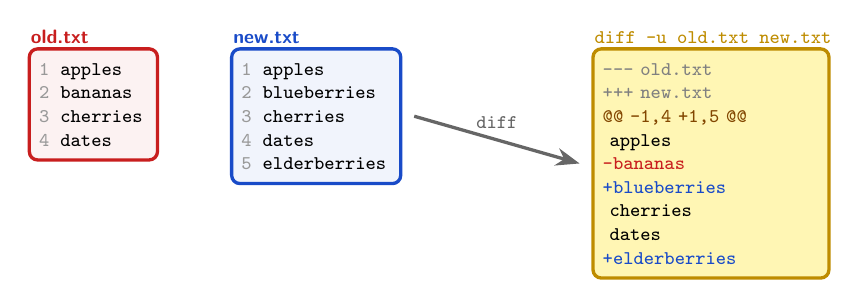
\begin{tikzpicture}[]
\matrix (o) [oldf, label={[oldlbl]north west:old.txt}, anchor=north west, at={(0,0)}, column 2/.style={nodes={text width=1.11cm}}] {
  |[ln]| 1 \amp \mbox{apples} \\
  |[ln]| 2 \amp \mbox{bananas} \\
  |[ln]| 3 \amp \mbox{cherries} \\
  |[ln]| 4 \amp \mbox{dates} \\
};
\matrix (n) [newf, label={[newlbl]north west:new.txt}, anchor=north west, at={($(o.north east)+(0.9,0)$)}, column 2/.style={nodes={text width=1.63cm}}] {
  |[ln]| 1 \amp \mbox{apples} \\
  |[ln]| 2 \amp \mbox{blueberries} \\
  |[ln]| 3 \amp \mbox{cherries} \\
  |[ln]| 4 \amp \mbox{dates} \\
  |[ln]| 5 \amp \mbox{elderberries} \\
};
\matrix (d) [difff, label={[difflbl]north west:diff -u old.txt new.txt}, anchor=north west, at={($(n.north east)+(2.4,0)$)}, column 1/.style={nodes={text width=2.75cm}}] {
  |[hdr]| \mbox{-{}-{}-{}\ old.txt} \\
  |[hdr]| \mbox{+++\ new.txt} \\
  |[hunk]| \mbox{@@\ -{}1,4\ +1,5\ @@} \\
  \mbox{\ apples} \\
  |[del]| \mbox{-{}bananas} \\
  |[add]| \mbox{+blueberries} \\
  \mbox{\ cherries} \\
  \mbox{\ dates} \\
  |[add]| \mbox{+elderberries} \\
};
\draw[bigarrow] ($(n.east)+(0.15,0)$) -- node[above, font=\scriptsize\ttfamily]{diff} ($(d.west)+(-0.15,0)$);
\end{tikzpicture}
\end{center}
\vspace{-0.6em}
\vspace{-0.3em}
\begin{columns}[T]
  \begin{column}{0.5\textwidth}
    \begin{itemize}\small
      \item \textcolor{oldred}{\textbf{Red rectangle}}: the old file
      \item \textcolor{newblue}{\textbf{Blue rectangle}}: the new file
      \item \textcolor{diffborder}{\textbf{Yellow rectangle}}: the diff between them
    \end{itemize}
  \end{column}
  \begin{column}{0.47\textwidth}
    \begin{itemize}\small
      \item Inside the diff, \textcolor{oldred}{\textbf{red lines}} exist only in the old file,
            \textcolor{newblue}{\textbf{blue lines}} only in the new file
      \item Black lines are in both: \textbf{context}
    \end{itemize}
  \end{column}
\end{columns}
\end{frame}
% ~~~~~~~~~~~~~~~~~~~~~~~~~~~~~~~~~~~~~~ A

% ~~~~~~~~~~~~~~~~~~~~~~~~~~~~~~~~~~~~~~ V
\section[Formats]{Reading a Diff}
% ~~~~~~~~~~~~~~~~~~~~~~~~~~~~~~~~~~~~~~ A

% ~~~~~~~~~~~~~~~~~~~~~~~~~~~~~~~~~~~~~~ V
\begin{frame}[t,fragile] \frametitle{The classic format: \texttt{diff old new}}
\vspace{-0.2em}
\begin{center}
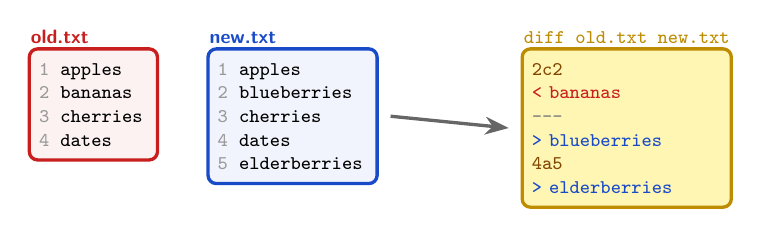
\begin{tikzpicture}[]
\matrix (o) [oldf, label={[oldlbl]north west:old.txt}, anchor=north west, at={(0,0)}, column 2/.style={nodes={text width=1.11cm}}] {
  |[ln]| 1 \amp \mbox{apples} \\
  |[ln]| 2 \amp \mbox{bananas} \\
  |[ln]| 3 \amp \mbox{cherries} \\
  |[ln]| 4 \amp \mbox{dates} \\
};
\matrix (n) [newf, label={[newlbl]north west:new.txt}, anchor=north west, at={($(o.north east)+(0.6,0)$)}, column 2/.style={nodes={text width=1.63cm}}] {
  |[ln]| 1 \amp \mbox{apples} \\
  |[ln]| 2 \amp \mbox{blueberries} \\
  |[ln]| 3 \amp \mbox{cherries} \\
  |[ln]| 4 \amp \mbox{dates} \\
  |[ln]| 5 \amp \mbox{elderberries} \\
};
\matrix (d) [difff, label={[difflbl]north west:diff old.txt new.txt}, anchor=north west, at={($(n.north east)+(1.8,0)$)}, column 1/.style={nodes={text width=2.41cm}}] {
  |[hunk]| \mbox{2c2} \\
  |[del]| \mbox{<\ bananas} \\
  |[hdr]| \mbox{-{}-{}-{}} \\
  |[add]| \mbox{>\ blueberries} \\
  |[hunk]| \mbox{4a5} \\
  |[add]| \mbox{>\ elderberries} \\
};
\draw[bigarrow] ($(n.east)+(0.15,0)$) -- ($(d.west)+(-0.15,0)$);
\end{tikzpicture}
\end{center}
\vspace{-0.6em}
\small
\begin{tabular}{@{}L{0.2\textwidth}L{0.74\textwidth}@{}}
  \toprule
  \textbf{Line} & \textbf{Meaning} \\
  \midrule
  \texttt{\textcolor{hunkc}{\textbf{2c2}}} & \textbf{c}hange old line 2 into new line 2 \\
  \texttt{\textcolor{oldred}{< bananas}} & the old line (from the \textcolor{oldred}{red} file) \\
  \texttt{\textcolor{gray}{-{}-{}-}} & separator between old and new \\
  \texttt{\textcolor{newblue}{> blueberries}} & the new line (from the \textcolor{newblue}{blue} file) \\
  \texttt{\textcolor{hunkc}{\textbf{4a5}}} & after old line 4, \textbf{a}dd new line 5 (a \texttt{d} would mean \textbf{d}elete) \\
  \bottomrule
\end{tabular}

\vspace{0.3em}
The classic format is a list of \emph{edit instructions}: change, add, delete.
\end{frame}
% ~~~~~~~~~~~~~~~~~~~~~~~~~~~~~~~~~~~~~~ A

% ~~~~~~~~~~~~~~~~~~~~~~~~~~~~~~~~~~~~~~ V
\begin{frame}[t,fragile] \frametitle{The unified format: \texttt{diff -u old new}}
\vspace{-0.2em}
\begin{center}
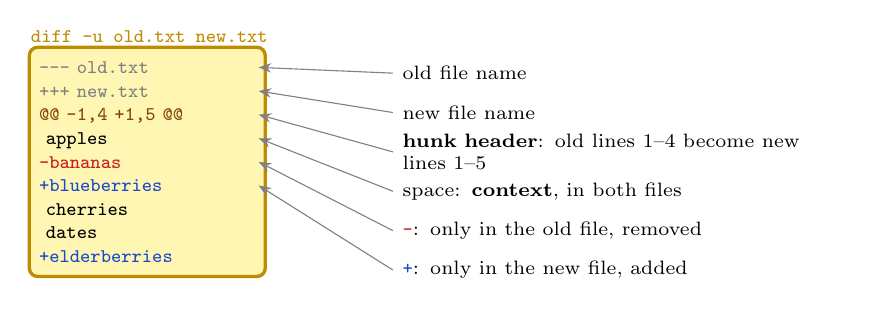
\begin{tikzpicture}[]
\matrix (d) [difff, label={[difflbl]north west:diff -u old.txt new.txt}, anchor=north west, at={(0,0)}, column 1/.style={nodes={text width=2.75cm}}] {
  |[hdr]| \mbox{-{}-{}-{}\ old.txt} \\
  |[hdr]| \mbox{+++\ new.txt} \\
  |[hunk]| \mbox{@@\ -{}1,4\ +1,5\ @@} \\
  \mbox{\ apples} \\
  |[del]| \mbox{-{}bananas} \\
  |[add]| \mbox{+blueberries} \\
  \mbox{\ cherries} \\
  \mbox{\ dates} \\
  |[add]| \mbox{+elderberries} \\
};
\node[note] (a0) at ($(d.north east)+(1.6,-0.35)$) {old file name};
\draw[notearrow] (a0.west) -- (d-1-1.east);
\node[note] (a1) at ($(d.north east)+(1.6,-0.85)$) {new file name};
\draw[notearrow] (a1.west) -- (d-2-1.east);
\node[note] (a2) at ($(d.north east)+(1.6,-1.35)$) {\textbf{hunk header}: old lines 1--4 become new lines 1--5};
\draw[notearrow] (a2.west) -- (d-3-1.east);
\node[note] (a3) at ($(d.north east)+(1.6,-1.85)$) {space: \textbf{context}, in both files};
\draw[notearrow] (a3.west) -- (d-4-1.east);
\node[note] (a4) at ($(d.north east)+(1.6,-2.35)$) {\textcolor{oldred}{\texttt{-}}: only in the old file, removed};
\draw[notearrow] (a4.west) -- (d-5-1.east);
\node[note] (a5) at ($(d.north east)+(1.6,-2.85)$) {\textcolor{newblue}{\texttt{+}}: only in the new file, added};
\draw[notearrow] (a5.west) -- (d-6-1.east);
\end{tikzpicture}
\end{center}
\vspace{-0.6em}
\begin{block}{Unified format (\texttt{diff -u})}
  This is the format Git uses. Instead of instructions, it shows the old and new lines
  \emph{in place}, surrounded by a few unchanged lines so you can see where the change is.
\end{block}
\end{frame}
% ~~~~~~~~~~~~~~~~~~~~~~~~~~~~~~~~~~~~~~ A

% ~~~~~~~~~~~~~~~~~~~~~~~~~~~~~~~~~~~~~~ V
\section[How]{How Diff Finds Changes}
% ~~~~~~~~~~~~~~~~~~~~~~~~~~~~~~~~~~~~~~ A

% ~~~~~~~~~~~~~~~~~~~~~~~~~~~~~~~~~~~~~~ V
\begin{frame}[t,fragile] \frametitle{Matching lines: the longest common subsequence}
\vspace{-0.2em}
\begin{center}
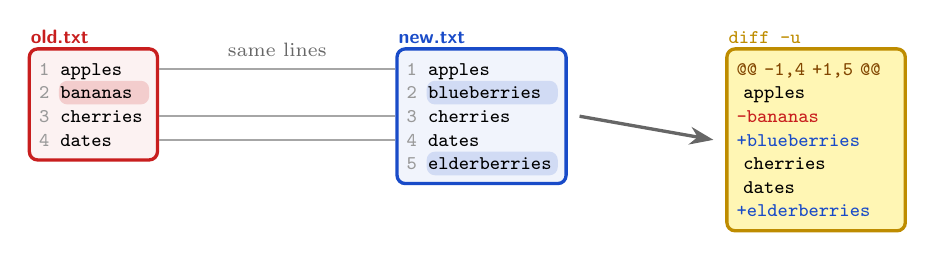
\begin{tikzpicture}[]
\matrix (o) [oldf, label={[oldlbl]north west:old.txt}, anchor=north west, at={(0,0)}, column 2/.style={nodes={text width=1.11cm}}] {
  |[ln]| 1 \amp \mbox{apples} \\
  |[ln]| 2 \amp |[hlold]| \mbox{bananas} \\
  |[ln]| 3 \amp \mbox{cherries} \\
  |[ln]| 4 \amp \mbox{dates} \\
};
\matrix (n) [newf, label={[newlbl]north west:new.txt}, anchor=north west, at={($(o.north east)+(3.0,0)$)}, column 2/.style={nodes={text width=1.63cm}}] {
  |[ln]| 1 \amp \mbox{apples} \\
  |[ln]| 2 \amp |[hlnew]| \mbox{blueberries} \\
  |[ln]| 3 \amp \mbox{cherries} \\
  |[ln]| 4 \amp \mbox{dates} \\
  |[ln]| 5 \amp |[hlnew]| \mbox{elderberries} \\
};
\matrix (d) [difff, label={[difflbl]north west:diff -u}, anchor=north west, at={($(n.north east)+(2.0,0)$)}, column 1/.style={nodes={text width=2.02cm}}] {
  |[hunk]| \mbox{@@\ -{}1,4\ +1,5\ @@} \\
  \mbox{\ apples} \\
  |[del]| \mbox{-{}bananas} \\
  |[add]| \mbox{+blueberries} \\
  \mbox{\ cherries} \\
  \mbox{\ dates} \\
  |[add]| \mbox{+elderberries} \\
};
\draw[bigarrow] ($(n.east)+(0.15,0)$) -- ($(d.west)+(-0.15,0)$);
\draw[match] (o.east |- o-1-2) -- (n.west |- n-1-2);
\draw[match] (o.east |- o-3-2) -- (n.west |- n-3-2);
\draw[match] (o.east |- o-4-2) -- (n.west |- n-4-2);
\node[font=\scriptsize, text=black!60] at ($(o.east |- o-1-2)!0.5!(n.west |- n-1-2)+(0,0.25)$) {same lines};
\end{tikzpicture}
\end{center}
\vspace{-0.6em}
\begin{enumerate}\small
  \item Find the \textbf{longest common subsequence} (LCS): the longest list of lines that
        appear in both files \emph{in the same order}. Here: \texttt{apples, cherries, dates}
  \item Lines in the LCS become \textbf{context} (black)
  \item Old lines not in the LCS become \textcolor{oldred}{\texttt{-} lines};
        new lines not in the LCS become \textcolor{newblue}{\texttt{+} lines}
\end{enumerate}
\small Real tools (Myers, patience, histogram algorithms) are fast ways to find a good LCS.
\end{frame}
% ~~~~~~~~~~~~~~~~~~~~~~~~~~~~~~~~~~~~~~ A

% ~~~~~~~~~~~~~~~~~~~~~~~~~~~~~~~~~~~~~~ V
\section[Code]{A Real Code Change}
% ~~~~~~~~~~~~~~~~~~~~~~~~~~~~~~~~~~~~~~ A

% ~~~~~~~~~~~~~~~~~~~~~~~~~~~~~~~~~~~~~~ V
\begin{frame}[t,fragile] \frametitle{A code change}
\vspace{-0.2em}
\begin{center}
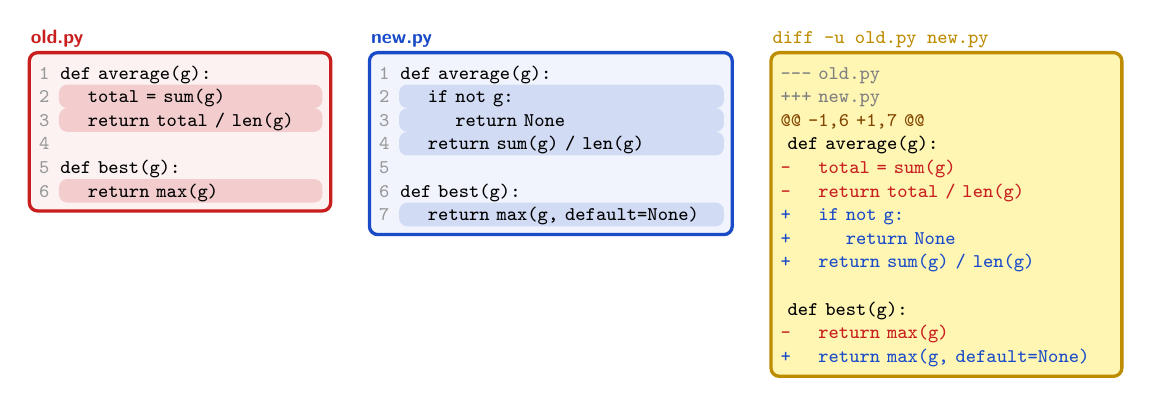
\begin{tikzpicture}[]
\matrix (o) [oldf, label={[oldlbl]north west:old.py}, anchor=north west, at={(0,0)}, column 2/.style={nodes={text width=3.31cm}}] {
  |[ln]| 1 \amp \mbox{def\ average(g):} \\
  |[ln]| 2 \amp |[hlold]| \mbox{\ \ \ \ total\ =\ sum(g)} \\
  |[ln]| 3 \amp |[hlold]| \mbox{\ \ \ \ return\ total\ /\ len(g)} \\
  |[ln]| 4 \amp \mbox{} \\
  |[ln]| 5 \amp \mbox{def\ best(g):} \\
  |[ln]| 6 \amp |[hlold]| \mbox{\ \ \ \ return\ max(g)} \\
};
\matrix (n) [newf, label={[newlbl]north west:new.py}, anchor=north west, at={($(o.north east)+(0.45,0)$)}, column 2/.style={nodes={text width=4.09cm}}] {
  |[ln]| 1 \amp \mbox{def\ average(g):} \\
  |[ln]| 2 \amp |[hlnew]| \mbox{\ \ \ \ if\ not\ g:} \\
  |[ln]| 3 \amp |[hlnew]| \mbox{\ \ \ \ \ \ \ \ return\ None} \\
  |[ln]| 4 \amp |[hlnew]| \mbox{\ \ \ \ return\ sum(g)\ /\ len(g)} \\
  |[ln]| 5 \amp \mbox{} \\
  |[ln]| 6 \amp \mbox{def\ best(g):} \\
  |[ln]| 7 \amp |[hlnew]| \mbox{\ \ \ \ return\ max(g,\ default=None)} \\
};
\matrix (d) [difff, label={[difflbl]north west:diff -u old.py new.py}, anchor=north west, at={($(n.north east)+(0.45,0)$)}, column 1/.style={nodes={text width=4.21cm}}] {
  |[hdr]| \mbox{-{}-{}-{}\ old.py} \\
  |[hdr]| \mbox{+++\ new.py} \\
  |[hunk]| \mbox{@@\ -{}1,6\ +1,7\ @@} \\
  \mbox{\ def\ average(g):} \\
  |[del]| \mbox{-{}\ \ \ \ total\ =\ sum(g)} \\
  |[del]| \mbox{-{}\ \ \ \ return\ total\ /\ len(g)} \\
  |[add]| \mbox{+\ \ \ \ if\ not\ g:} \\
  |[add]| \mbox{+\ \ \ \ \ \ \ \ return\ None} \\
  |[add]| \mbox{+\ \ \ \ return\ sum(g)\ /\ len(g)} \\
  \mbox{\ } \\
  \mbox{\ def\ best(g):} \\
  |[del]| \mbox{-{}\ \ \ \ return\ max(g)} \\
  |[add]| \mbox{+\ \ \ \ return\ max(g,\ default=None)} \\
};
\end{tikzpicture}
\end{center}
\vspace{-0.6em}
\vspace{-0.2em}
\small
\begin{itemize}
  \item Two separate edits, but only \textbf{one hunk}: \texttt{diff -u} keeps 3 lines of
        context around each edit, and here the two context windows overlap
  \item \texttt{@@ -1,6 +1,7 @@}: 6 old lines became 7 new lines (3 removed, 4 added)
\end{itemize}
\end{frame}
% ~~~~~~~~~~~~~~~~~~~~~~~~~~~~~~~~~~~~~~ A

% ~~~~~~~~~~~~~~~~~~~~~~~~~~~~~~~~~~~~~~ V
\begin{frame}[t,fragile] \frametitle{Hunks and line numbers}
\vspace{-0.2em}
\begin{center}
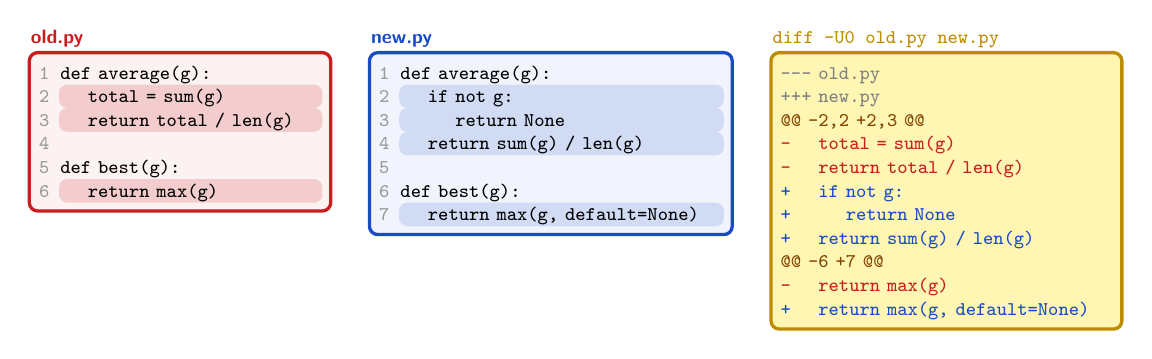
\begin{tikzpicture}[]
\matrix (o) [oldf, label={[oldlbl]north west:old.py}, anchor=north west, at={(0,0)}, column 2/.style={nodes={text width=3.31cm}}] {
  |[ln]| 1 \amp \mbox{def\ average(g):} \\
  |[ln]| 2 \amp |[hlold]| \mbox{\ \ \ \ total\ =\ sum(g)} \\
  |[ln]| 3 \amp |[hlold]| \mbox{\ \ \ \ return\ total\ /\ len(g)} \\
  |[ln]| 4 \amp \mbox{} \\
  |[ln]| 5 \amp \mbox{def\ best(g):} \\
  |[ln]| 6 \amp |[hlold]| \mbox{\ \ \ \ return\ max(g)} \\
};
\matrix (n) [newf, label={[newlbl]north west:new.py}, anchor=north west, at={($(o.north east)+(0.45,0)$)}, column 2/.style={nodes={text width=4.09cm}}] {
  |[ln]| 1 \amp \mbox{def\ average(g):} \\
  |[ln]| 2 \amp |[hlnew]| \mbox{\ \ \ \ if\ not\ g:} \\
  |[ln]| 3 \amp |[hlnew]| \mbox{\ \ \ \ \ \ \ \ return\ None} \\
  |[ln]| 4 \amp |[hlnew]| \mbox{\ \ \ \ return\ sum(g)\ /\ len(g)} \\
  |[ln]| 5 \amp \mbox{} \\
  |[ln]| 6 \amp \mbox{def\ best(g):} \\
  |[ln]| 7 \amp |[hlnew]| \mbox{\ \ \ \ return\ max(g,\ default=None)} \\
};
\matrix (d) [difff, label={[difflbl]north west:diff -U0 old.py new.py}, anchor=north west, at={($(n.north east)+(0.45,0)$)}, column 1/.style={nodes={text width=4.21cm}}] {
  |[hdr]| \mbox{-{}-{}-{}\ old.py} \\
  |[hdr]| \mbox{+++\ new.py} \\
  |[hunk]| \mbox{@@\ -{}2,2\ +2,3\ @@} \\
  |[del]| \mbox{-{}\ \ \ \ total\ =\ sum(g)} \\
  |[del]| \mbox{-{}\ \ \ \ return\ total\ /\ len(g)} \\
  |[add]| \mbox{+\ \ \ \ if\ not\ g:} \\
  |[add]| \mbox{+\ \ \ \ \ \ \ \ return\ None} \\
  |[add]| \mbox{+\ \ \ \ return\ sum(g)\ /\ len(g)} \\
  |[hunk]| \mbox{@@\ -{}6\ +7\ @@} \\
  |[del]| \mbox{-{}\ \ \ \ return\ max(g)} \\
  |[add]| \mbox{+\ \ \ \ return\ max(g,\ default=None)} \\
};
\end{tikzpicture}
\end{center}
\vspace{-0.6em}
\vspace{-0.2em}
\small
With \textbf{no context} (\texttt{-U0}) the two edits become two hunks.
Headers read \texttt{-\textcolor{oldred}{start,count}\ +\textcolor{newblue}{start,count}}:

\begin{tabular}{@{}L{0.24\textwidth}L{0.7\textwidth}@{}}
  \texttt{@@ -\textcolor{oldred}{2,2} +\textcolor{newblue}{2,3} @@} &
    \textcolor{oldred}{old lines 2--3} (2 lines) are replaced by \textcolor{newblue}{new lines 2--4} (3 lines) \\
  \texttt{@@ -\textcolor{oldred}{6} +\textcolor{newblue}{7} @@} &
    \textcolor{oldred}{old line 6} is replaced by \textcolor{newblue}{new line 7} (a missing count means 1) \\
\end{tabular}

Old line 6 is new line 7 because the first hunk added a line, shifting everything below it.
\end{frame}
% ~~~~~~~~~~~~~~~~~~~~~~~~~~~~~~~~~~~~~~ A

% ~~~~~~~~~~~~~~~~~~~~~~~~~~~~~~~~~~~~~~ V
\begin{frame}[t,fragile] \frametitle{What Git adds: the header}
\vspace{-0.2em}
\begin{center}
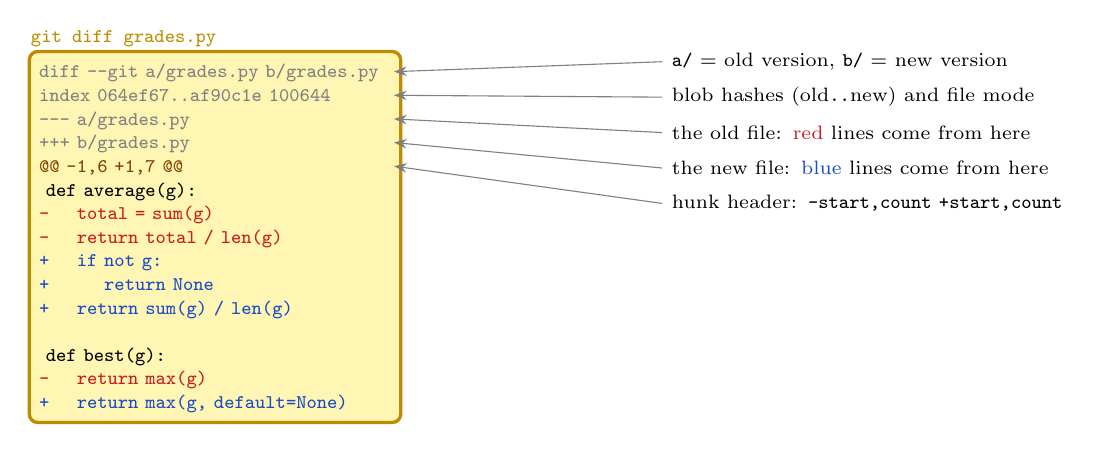
\begin{tikzpicture}[]
\matrix (d) [difff, label={[difflbl]north west:git diff grades.py}, anchor=north west, at={(0,0)}, column 1/.style={nodes={text width=4.47cm}}] {
  |[hdr]| \mbox{diff\ -{}-{}git\ a/grades.py\ b/grades.py} \\
  |[hdr]| \mbox{index\ 064ef67..af90c1e\ 100644} \\
  |[hdr]| \mbox{-{}-{}-{}\ a/grades.py} \\
  |[hdr]| \mbox{+++\ b/grades.py} \\
  |[hunk]| \mbox{@@\ -{}1,6\ +1,7\ @@} \\
  \mbox{\ def\ average(g):} \\
  |[del]| \mbox{-{}\ \ \ \ total\ =\ sum(g)} \\
  |[del]| \mbox{-{}\ \ \ \ return\ total\ /\ len(g)} \\
  |[add]| \mbox{+\ \ \ \ if\ not\ g:} \\
  |[add]| \mbox{+\ \ \ \ \ \ \ \ return\ None} \\
  |[add]| \mbox{+\ \ \ \ return\ sum(g)\ /\ len(g)} \\
  \mbox{\ } \\
  \mbox{\ def\ best(g):} \\
  |[del]| \mbox{-{}\ \ \ \ return\ max(g)} \\
  |[add]| \mbox{+\ \ \ \ return\ max(g,\ default=None)} \\
};
\node[note, text width=5.2cm] (a0) at ($(d.north east)+(3.3,-0.15)$) {\texttt{a/} = old version, \texttt{b/} = new version};
\draw[notearrow] (a0.west) -- (d-1-1.east);
\node[note, text width=5.2cm] (a1) at ($(d.north east)+(3.3,-0.6)$) {blob hashes (old\texttt{..}new) and file mode};
\draw[notearrow] (a1.west) -- (d-2-1.east);
\node[note, text width=5.2cm] (a2) at ($(d.north east)+(3.3,-1.05)$) {the old file: \textcolor{oldred}{red} lines come from here};
\draw[notearrow] (a2.west) -- (d-3-1.east);
\node[note, text width=5.2cm] (a3) at ($(d.north east)+(3.3,-1.5)$) {the new file: \textcolor{newblue}{blue} lines come from here};
\draw[notearrow] (a3.west) -- (d-4-1.east);
\node[note, text width=5.2cm] (a4) at ($(d.north east)+(3.3,-1.95)$) {hunk header: \texttt{-start,count +start,count}};
\draw[notearrow] (a4.west) -- (d-5-1.east);
\end{tikzpicture}
\end{center}
\vspace{-0.6em}
\small From the first \texttt{@@} on, it is the same unified diff; Git adds two lines of bookkeeping on top.
\end{frame}
% ~~~~~~~~~~~~~~~~~~~~~~~~~~~~~~~~~~~~~~ A

% ~~~~~~~~~~~~~~~~~~~~~~~~~~~~~~~~~~~~~~ V
\section[Details]{Details That Matter}
% ~~~~~~~~~~~~~~~~~~~~~~~~~~~~~~~~~~~~~~ A

% ~~~~~~~~~~~~~~~~~~~~~~~~~~~~~~~~~~~~~~ V
\begin{frame}[t,fragile] \frametitle{Diffs are line-based}
\vspace{-0.2em}
\begin{center}
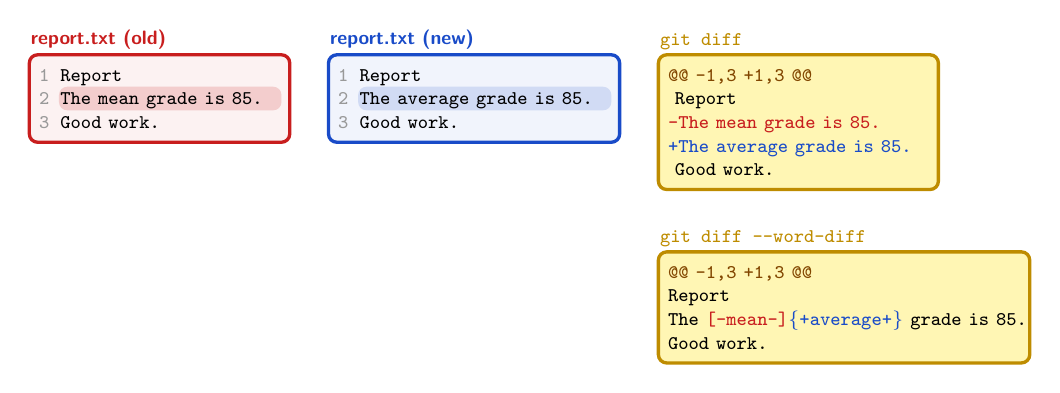
\begin{tikzpicture}[]
\matrix (o) [oldf, label={[oldlbl]north west:report.txt (old)}, anchor=north west, at={(0,0)}, column 2/.style={nodes={text width=2.79cm}}] {
  |[ln]| 1 \amp \mbox{Report} \\
  |[ln]| 2 \amp |[hlold]| \mbox{The\ mean\ grade\ is\ 85.} \\
  |[ln]| 3 \amp \mbox{Good\ work.} \\
};
\matrix (n) [newf, label={[newlbl]north west:report.txt (new)}, anchor=north west, at={($(o.north east)+(0.45,0)$)}, column 2/.style={nodes={text width=3.18cm}}] {
  |[ln]| 1 \amp \mbox{Report} \\
  |[ln]| 2 \amp |[hlnew]| \mbox{The\ average\ grade\ is\ 85.} \\
  |[ln]| 3 \amp \mbox{Good\ work.} \\
};
\matrix (d) [difff, label={[difflbl]north west:git diff}, anchor=north west, at={($(n.north east)+(0.45,0)$)}, column 1/.style={nodes={text width=3.31cm}}] {
  |[hunk]| \mbox{@@\ -{}1,3\ +1,3\ @@} \\
  \mbox{\ Report} \\
  |[del]| \mbox{-{}The\ mean\ grade\ is\ 85.} \\
  |[add]| \mbox{+The\ average\ grade\ is\ 85.} \\
  \mbox{\ Good\ work.} \\
};
\matrix (w) [difff, label={[difflbl]north west:git diff --word-diff}, anchor=north west, at={($(d.south west)+(0,-0.75)$)}, column 1/.style={nodes={text width=4.47cm}}] {
  |[hunk]| \mbox{@@\ -{}1,3\ +1,3\ @@} \\
  \mbox{Report} \\
  \mbox{The\ \textcolor{oldred}{[-{}mean-{}]}\textcolor{newblue}{\{+average+\}}\ grade\ is\ 85.} \\
  \mbox{Good\ work.} \\
};
\end{tikzpicture}
\end{center}
\vspace{-0.6em}
\small
\begin{itemize}
  \item Diffs work on \textbf{whole lines}: one changed word replaces the entire line
  \item \texttt{--word-diff} shows which words changed:
        \textcolor{oldred}{\texttt{[-removed-]}} \textcolor{newblue}{\texttt{\{+added+\}}}.
        Very useful for prose, \LaTeX{} and long lines
\end{itemize}
\end{frame}
% ~~~~~~~~~~~~~~~~~~~~~~~~~~~~~~~~~~~~~~ A

% ~~~~~~~~~~~~~~~~~~~~~~~~~~~~~~~~~~~~~~ V
\begin{frame}[t,fragile] \frametitle{Whitespace counts}
\vspace{-0.2em}
\begin{center}
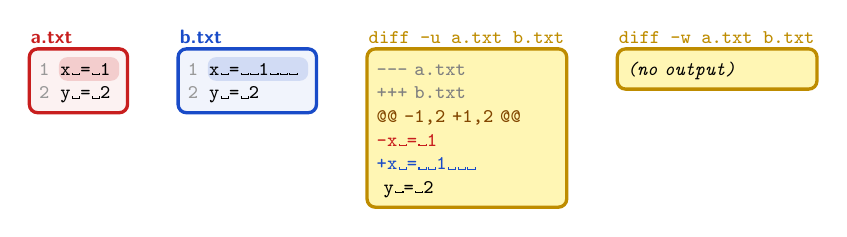
\begin{tikzpicture}[]
\matrix (o) [oldf, label={[oldlbl]north west:a.txt}, anchor=north west, at={(0,0)}, column 2/.style={nodes={text width=0.73cm}}] {
  |[ln]| 1 \amp |[hlold]| \mbox{x\textvisiblespace{}=\textvisiblespace{}1} \\
  |[ln]| 2 \amp \mbox{y\textvisiblespace{}=\textvisiblespace{}2} \\
};
\matrix (n) [newf, label={[newlbl]north west:b.txt}, anchor=north west, at={($(o.north east)+(0.6,0)$)}, column 2/.style={nodes={text width=1.24cm}}] {
  |[ln]| 1 \amp |[hlnew]| \mbox{x\textvisiblespace{}=\textvisiblespace{}\textvisiblespace{}1\textvisiblespace{}\textvisiblespace{}\textvisiblespace{}} \\
  |[ln]| 2 \amp \mbox{y\textvisiblespace{}=\textvisiblespace{}2} \\
};
\matrix (d) [difff, label={[difflbl]north west:diff -u a.txt b.txt}, anchor=north west, at={($(n.north east)+(0.6,0)$)}, column 1/.style={nodes={text width=2.29cm}}] {
  |[hdr]| \mbox{-{}-{}-{}\ a.txt} \\
  |[hdr]| \mbox{+++\ b.txt} \\
  |[hunk]| \mbox{@@\ -{}1,2\ +1,2\ @@} \\
  |[del]| \mbox{-{}x\textvisiblespace{}=\textvisiblespace{}1} \\
  |[add]| \mbox{+x\textvisiblespace{}=\textvisiblespace{}\textvisiblespace{}1\textvisiblespace{}\textvisiblespace{}\textvisiblespace{}} \\
  \mbox{\ y\textvisiblespace{}=\textvisiblespace{}2} \\
};
\matrix (e) [difff, label={[difflbl]north west:diff -w a.txt b.txt}, anchor=north west, at={($(d.north east)+(0.6,0)$)}, column 1/.style={nodes={text width=2.29cm}}] {
  \textit{(no output)} \\
};
\end{tikzpicture}
\end{center}
\vspace{-0.6em}
\small
\begin{itemize}
  \item \texttt{\textvisiblespace} marks a space. The two files look the same on screen,
        but line 1 has an extra space and three trailing spaces
  \item For \texttt{diff} that is a real change. \texttt{diff -w} (and \texttt{git diff -w})
        ignores whitespace, so it reports nothing
  \item Invisible whitespace changes are a common source of noisy diffs and needless conflicts
\end{itemize}
\end{frame}
% ~~~~~~~~~~~~~~~~~~~~~~~~~~~~~~~~~~~~~~ A

% ~~~~~~~~~~~~~~~~~~~~~~~~~~~~~~~~~~~~~~ V
\begin{frame}[t,fragile] \frametitle{New and deleted files}
\vspace{-0.2em}
\begin{center}
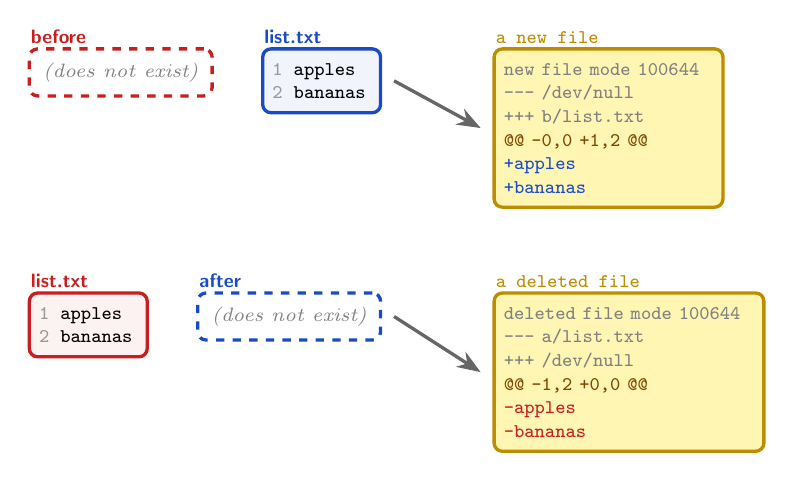
\begin{tikzpicture}[]
\node[nofile, draw=oldred, anchor=north west] (o1) at (0,0) {(does not exist)};
\node[oldlbl, anchor=south west] at (o1.north west) {before};
\matrix (n1) [newf, label={[newlbl]north west:list.txt}, anchor=north west, at={($(o1.north east)+(0.6,0)$)}, column 2/.style={nodes={text width=0.98cm}}] {
  |[ln]| 1 \amp \mbox{apples} \\
  |[ln]| 2 \amp \mbox{bananas} \\
};
\matrix (d1) [difff, label={[difflbl]north west:a new file}, anchor=north west, at={($(n1.north east)+(1.4,0)$)}, column 1/.style={nodes={text width=2.66cm}}] {
  |[hdr]| \mbox{new\ file\ mode\ 100644} \\
  |[hdr]| \mbox{-{}-{}-{}\ /dev/null} \\
  |[hdr]| \mbox{+++\ b/list.txt} \\
  |[hunk]| \mbox{@@\ -{}0,0\ +1,2\ @@} \\
  |[add]| \mbox{+apples} \\
  |[add]| \mbox{+bananas} \\
};
\draw[bigarrow] ($(n1.east)+(0.15,0)$) -- ($(d1.west)+(-0.15,0)$);
\matrix (o2) [oldf, label={[oldlbl]north west:list.txt}, anchor=north west, at={(0,-3.1)}, column 2/.style={nodes={text width=0.98cm}}] {
  |[ln]| 1 \amp \mbox{apples} \\
  |[ln]| 2 \amp \mbox{bananas} \\
};
\node[nofile, draw=newblue, anchor=north west] (n2) at ($(o2.north east)+(0.6,0)$) {(does not exist)};
\node[newlbl, anchor=south west] at (n2.north west) {after};
\matrix (d2) [difff, label={[difflbl]north west:a deleted file}, anchor=north west, at={($(d1.north west)+(0,-3.1)$)}, column 1/.style={nodes={text width=3.18cm}}] {
  |[hdr]| \mbox{deleted\ file\ mode\ 100644} \\
  |[hdr]| \mbox{-{}-{}-{}\ a/list.txt} \\
  |[hdr]| \mbox{+++\ /dev/null} \\
  |[hunk]| \mbox{@@\ -{}1,2\ +0,0\ @@} \\
  |[del]| \mbox{-{}apples} \\
  |[del]| \mbox{-{}bananas} \\
};
\draw[bigarrow] ($(n2.east)+(0.15,0)$) -- ($(d2.west)+(-0.15,0)$);
\end{tikzpicture}
\end{center}
\vspace{-0.6em}
\small A missing file is treated as \textbf{empty} (\texttt{/dev/null}). A new file is all
\textcolor{newblue}{\texttt{+}} lines; a deleted file is all \textcolor{oldred}{\texttt{-}} lines.
\texttt{@@ -0,0 +1,2 @@} means ``0 old lines become 2 new lines''.
\end{frame}
% ~~~~~~~~~~~~~~~~~~~~~~~~~~~~~~~~~~~~~~ A

% ~~~~~~~~~~~~~~~~~~~~~~~~~~~~~~~~~~~~~~ V
\section[Apply]{Applying a Diff}
% ~~~~~~~~~~~~~~~~~~~~~~~~~~~~~~~~~~~~~~ A

% ~~~~~~~~~~~~~~~~~~~~~~~~~~~~~~~~~~~~~~ V
\begin{frame}[t,fragile] \frametitle{Old + diff = new}
\vspace{-0.2em}
\begin{center}
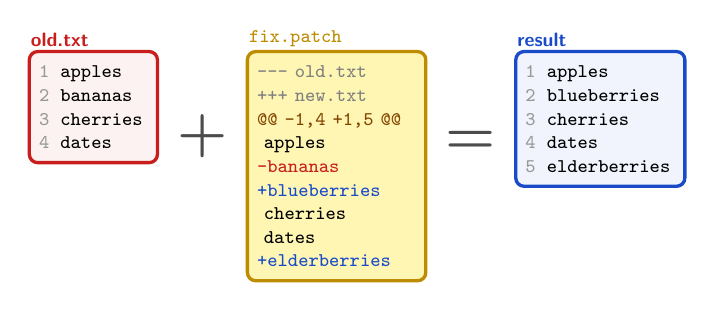
\begin{tikzpicture}[]
\matrix (o) [oldf, label={[oldlbl]north west:old.txt}, anchor=north west, at={(0,0)}, column 2/.style={nodes={text width=1.11cm}}] {
  |[ln]| 1 \amp \mbox{apples} \\
  |[ln]| 2 \amp \mbox{bananas} \\
  |[ln]| 3 \amp \mbox{cherries} \\
  |[ln]| 4 \amp \mbox{dates} \\
};
\matrix (d) [difff, label={[difflbl]north west:fix.patch}, anchor=north west, at={($(o.north east)+(1.1,0)$)}, column 1/.style={nodes={text width=2.02cm}}] {
  |[hdr]| \mbox{-{}-{}-{}\ old.txt} \\
  |[hdr]| \mbox{+++\ new.txt} \\
  |[hunk]| \mbox{@@\ -{}1,4\ +1,5\ @@} \\
  \mbox{\ apples} \\
  |[del]| \mbox{-{}bananas} \\
  |[add]| \mbox{+blueberries} \\
  \mbox{\ cherries} \\
  \mbox{\ dates} \\
  |[add]| \mbox{+elderberries} \\
};
\matrix (n) [newf, label={[newlbl]north west:result}, anchor=north west, at={($(d.north east)+(1.1,0)$)}, column 2/.style={nodes={text width=1.63cm}}] {
  |[ln]| 1 \amp \mbox{apples} \\
  |[ln]| 2 \amp \mbox{blueberries} \\
  |[ln]| 3 \amp \mbox{cherries} \\
  |[ln]| 4 \amp \mbox{dates} \\
  |[ln]| 5 \amp \mbox{elderberries} \\
};
\node[font=\huge\bfseries, text=black!70] (p) at ($(o.east)!0.5!(d.west)$) {+};
\node[font=\huge\bfseries, text=black!70] (e) at ($(d.east)!0.5!(n.west)$) {=};
\end{tikzpicture}
\end{center}
\vspace{-0.6em}
\begin{lstlisting}
diff -u old.txt new.txt > fix.patch   # save the diff: it is now a "patch"
patch old.txt < fix.patch             # patching file old.txt   (it now equals new.txt)
git apply fix.patch                   # the same idea inside a Git repository
\end{lstlisting}
\small A diff is a \textbf{recipe}: given the old file, it rebuilds the new one.
That is how patches are sent by e-mail, and how Git replays commits during a rebase.
\end{frame}
% ~~~~~~~~~~~~~~~~~~~~~~~~~~~~~~~~~~~~~~ A

% ~~~~~~~~~~~~~~~~~~~~~~~~~~~~~~~~~~~~~~ V
\begin{frame}[t,fragile] \frametitle{New $-$ diff = old}
\vspace{-0.2em}
\begin{center}
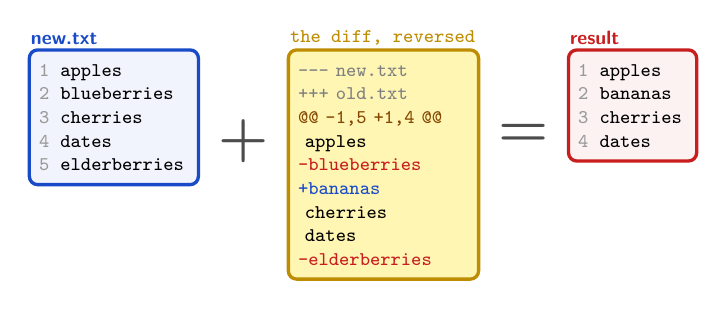
\begin{tikzpicture}[]
\matrix (n) [newf, label={[newlbl]north west:new.txt}, anchor=north west, at={(0,0)}, column 2/.style={nodes={text width=1.63cm}}] {
  |[ln]| 1 \amp \mbox{apples} \\
  |[ln]| 2 \amp \mbox{blueberries} \\
  |[ln]| 3 \amp \mbox{cherries} \\
  |[ln]| 4 \amp \mbox{dates} \\
  |[ln]| 5 \amp \mbox{elderberries} \\
};
\matrix (d) [difff, label={[difflbl]north west:the diff, reversed}, anchor=north west, at={($(n.north east)+(1.1,0)$)}, column 1/.style={nodes={text width=2.17cm}}] {
  |[hdr]| \mbox{-{}-{}-{}\ new.txt} \\
  |[hdr]| \mbox{+++\ old.txt} \\
  |[hunk]| \mbox{@@\ -{}1,5\ +1,4\ @@} \\
  \mbox{\ apples} \\
  |[del]| \mbox{-{}blueberries} \\
  |[add]| \mbox{+bananas} \\
  \mbox{\ cherries} \\
  \mbox{\ dates} \\
  |[del]| \mbox{-{}elderberries} \\
};
\matrix (o) [oldf, label={[oldlbl]north west:result}, anchor=north west, at={($(d.north east)+(1.1,0)$)}, column 2/.style={nodes={text width=1.11cm}}] {
  |[ln]| 1 \amp \mbox{apples} \\
  |[ln]| 2 \amp \mbox{bananas} \\
  |[ln]| 3 \amp \mbox{cherries} \\
  |[ln]| 4 \amp \mbox{dates} \\
};
\node[font=\huge\bfseries, text=black!70] (p) at ($(n.east)!0.5!(d.west)$) {+};
\node[font=\huge\bfseries, text=black!70] (e) at ($(d.east)!0.5!(o.west)$) {=};
\end{tikzpicture}
\end{center}
\vspace{-0.6em}
\begin{lstlisting}
patch -R new.txt < fix.patch          # -R: apply the patch in reverse (new.txt -> old.txt)
\end{lstlisting}
\small
\begin{itemize}
  \item Reversing a diff swaps \texttt{-} and \texttt{+}, and swaps the numbers in the hunk header.
        The colors stay with their file: \textcolor{newblue}{blue lines} are now removed,
        \textcolor{oldred}{red lines} added back
  \item This is exactly what \texttt{git revert} does with a commit's diff
\end{itemize}
\end{frame}
% ~~~~~~~~~~~~~~~~~~~~~~~~~~~~~~~~~~~~~~ A

% ~~~~~~~~~~~~~~~~~~~~~~~~~~~~~~~~~~~~~~ V
\begin{frame}[t,fragile] \frametitle{Context finds the right place}
\vspace{-0.2em}
\begin{center}
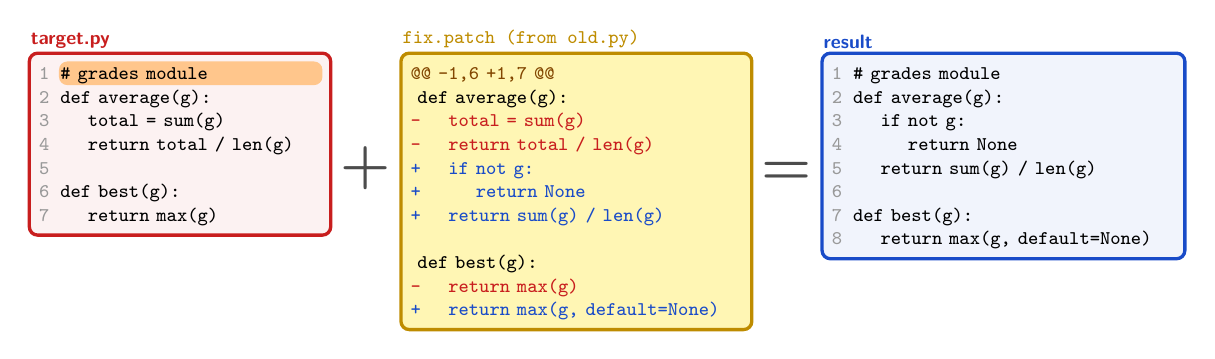
\begin{tikzpicture}[]
\matrix (o) [oldf, label={[oldlbl]north west:target.py}, anchor=north west, at={(0,0)}, column 2/.style={nodes={text width=3.31cm}}] {
  |[ln]| 1 \amp |[hlmis]| \mbox{\#\ grades\ module} \\
  |[ln]| 2 \amp \mbox{def\ average(g):} \\
  |[ln]| 3 \amp \mbox{\ \ \ \ total\ =\ sum(g)} \\
  |[ln]| 4 \amp \mbox{\ \ \ \ return\ total\ /\ len(g)} \\
  |[ln]| 5 \amp \mbox{} \\
  |[ln]| 6 \amp \mbox{def\ best(g):} \\
  |[ln]| 7 \amp \mbox{\ \ \ \ return\ max(g)} \\
};
\matrix (d) [difff, label={[difflbl]north west:fix.patch (from old.py)}, anchor=north west, at={($(o.north east)+(0.85,0)$)}, column 1/.style={nodes={text width=4.21cm}}] {
  |[hunk]| \mbox{@@\ -{}1,6\ +1,7\ @@} \\
  \mbox{\ def\ average(g):} \\
  |[del]| \mbox{-{}\ \ \ \ total\ =\ sum(g)} \\
  |[del]| \mbox{-{}\ \ \ \ return\ total\ /\ len(g)} \\
  |[add]| \mbox{+\ \ \ \ if\ not\ g:} \\
  |[add]| \mbox{+\ \ \ \ \ \ \ \ return\ None} \\
  |[add]| \mbox{+\ \ \ \ return\ sum(g)\ /\ len(g)} \\
  \mbox{\ } \\
  \mbox{\ def\ best(g):} \\
  |[del]| \mbox{-{}\ \ \ \ return\ max(g)} \\
  |[add]| \mbox{+\ \ \ \ return\ max(g,\ default=None)} \\
};
\matrix (n) [newf, label={[newlbl]north west:result}, anchor=north west, at={($(d.north east)+(0.85,0)$)}, column 2/.style={nodes={text width=4.09cm}}] {
  |[ln]| 1 \amp \mbox{\#\ grades\ module} \\
  |[ln]| 2 \amp \mbox{def\ average(g):} \\
  |[ln]| 3 \amp \mbox{\ \ \ \ if\ not\ g:} \\
  |[ln]| 4 \amp \mbox{\ \ \ \ \ \ \ \ return\ None} \\
  |[ln]| 5 \amp \mbox{\ \ \ \ return\ sum(g)\ /\ len(g)} \\
  |[ln]| 6 \amp \mbox{} \\
  |[ln]| 7 \amp \mbox{def\ best(g):} \\
  |[ln]| 8 \amp \mbox{\ \ \ \ return\ max(g,\ default=None)} \\
};
\node[font=\huge\bfseries, text=black!70] (p) at ($(o.east)!0.5!(d.west)$) {+};
\node[font=\huge\bfseries, text=black!70] (e) at ($(d.east)!0.5!(n.west)$) {=};
\end{tikzpicture}
\end{center}
\vspace{-0.6em}
\vspace{-0.3em}
\begin{lstlisting}[language={}]
$ patch target.py < fix.patch
Hunk #1 succeeded at 2 (offset 1 line).
\end{lstlisting}
\small The patch says ``line 1'', but \texttt{target.py} has an extra first line (orange).
\texttt{patch} searches for the \textbf{context lines} (black), finds them one line lower,
and applies the hunk there.
\end{frame}
% ~~~~~~~~~~~~~~~~~~~~~~~~~~~~~~~~~~~~~~ A

% ~~~~~~~~~~~~~~~~~~~~~~~~~~~~~~~~~~~~~~ V
\begin{frame}[t,fragile] \frametitle{When the lines don't match: a conflict}
\vspace{-0.2em}
\begin{center}
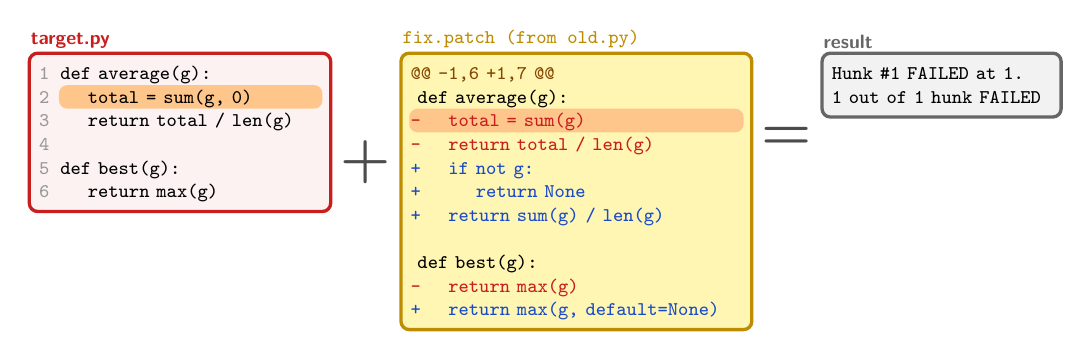
\begin{tikzpicture}[]
\matrix (o) [oldf, label={[oldlbl]north west:target.py}, anchor=north west, at={(0,0)}, column 2/.style={nodes={text width=3.31cm}}] {
  |[ln]| 1 \amp \mbox{def\ average(g):} \\
  |[ln]| 2 \amp |[hlmis]| \mbox{\ \ \ \ total\ =\ sum(g,\ 0)} \\
  |[ln]| 3 \amp \mbox{\ \ \ \ return\ total\ /\ len(g)} \\
  |[ln]| 4 \amp \mbox{} \\
  |[ln]| 5 \amp \mbox{def\ best(g):} \\
  |[ln]| 6 \amp \mbox{\ \ \ \ return\ max(g)} \\
};
\matrix (d) [difff, label={[difflbl]north west:fix.patch (from old.py)}, anchor=north west, at={($(o.north east)+(0.85,0)$)}, column 1/.style={nodes={text width=4.21cm}}] {
  |[hunk]| \mbox{@@\ -{}1,6\ +1,7\ @@} \\
  \mbox{\ def\ average(g):} \\
  |[del,hlmis]| \mbox{-{}\ \ \ \ total\ =\ sum(g)} \\
  |[del]| \mbox{-{}\ \ \ \ return\ total\ /\ len(g)} \\
  |[add]| \mbox{+\ \ \ \ if\ not\ g:} \\
  |[add]| \mbox{+\ \ \ \ \ \ \ \ return\ None} \\
  |[add]| \mbox{+\ \ \ \ return\ sum(g)\ /\ len(g)} \\
  \mbox{\ } \\
  \mbox{\ def\ best(g):} \\
  |[del]| \mbox{-{}\ \ \ \ return\ max(g)} \\
  |[add]| \mbox{+\ \ \ \ return\ max(g,\ default=None)} \\
};
\matrix (t) [termf, label={[termlbl]north west:result}, anchor=north west, at={($(d.north east)+(0.85,0)$)}, column 1/.style={nodes={text width=2.79cm}}] {
  \mbox{Hunk\ \#1\ FAILED\ at\ 1.} \\
  \mbox{1\ out\ of\ 1\ hunk\ FAILED} \\
};
\node[font=\huge\bfseries, text=black!70] (p) at ($(o.east)!0.5!(d.west)$) {+};
\node[font=\huge\bfseries, text=black!70] (e) at ($(d.east)!0.5!(t.west)$) {=};
\end{tikzpicture}
\end{center}
\vspace{-0.6em}
\small
\begin{itemize}
  \item The patch expects to remove \texttt{total = sum(g)}, but the file says
        \texttt{total = sum(g, 0)}: someone else changed that line
  \item The lines the diff wants to change are not there, so \texttt{patch} refuses
        rather than guess
  \item In Git this is a \textbf{conflict}: two diffs changed the same lines, and you
        must combine them by hand
\end{itemize}
\end{frame}
% ~~~~~~~~~~~~~~~~~~~~~~~~~~~~~~~~~~~~~~ A

% ~~~~~~~~~~~~~~~~~~~~~~~~~~~~~~~~~~~~~~ V
\section[Summary]{Summary}
% ~~~~~~~~~~~~~~~~~~~~~~~~~~~~~~~~~~~~~~ A

% ~~~~~~~~~~~~~~~~~~~~~~~~~~~~~~~~~~~~~~ V
\begin{frame}[t,fragile] \frametitle{Summary}
\vspace{-0.2em}
\begin{center}
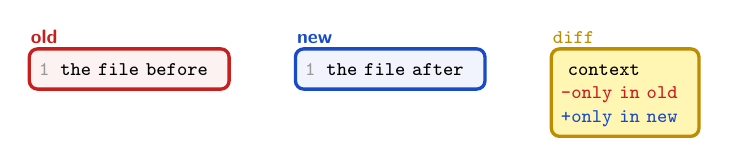
\begin{tikzpicture}[]
\matrix (o) [oldf, label={[oldlbl]north west:old}, anchor=north west, at={(0,0)}, column 2/.style={nodes={text width=2.02cm}}] {
  |[ln]| 1 \amp \mbox{the\ file\ before} \\
};
\matrix (n) [newf, label={[newlbl]north west:new}, anchor=north west, at={($(o.north east)+(0.8,0)$)}, column 2/.style={nodes={text width=1.89cm}}] {
  |[ln]| 1 \amp \mbox{the\ file\ after} \\
};
\matrix (d) [difff, label={[difflbl]north west:diff}, anchor=north west, at={($(n.north east)+(0.8,0)$)}, column 1/.style={nodes={text width=1.63cm}}] {
  \mbox{\ context} \\
  |[del]| \mbox{-{}only\ in\ old} \\
  |[add]| \mbox{+only\ in\ new} \\
};
\end{tikzpicture}
\end{center}
\vspace{-0.6em}
\small
\begin{tabular}{@{}L{0.46\textwidth}L{0.48\textwidth}@{}}
  \toprule
  \textbf{Idea} & \textbf{Example} \\
  \midrule
  A diff lists removed and added lines & \textcolor{oldred}{\texttt{-bananas}} \textcolor{newblue}{\texttt{+blueberries}} \\
  It is built from the longest common subsequence & common lines become context \\
  A hunk is one block of nearby changes & \texttt{@@ -2,2 +2,3 @@} \\
  Diffs are line-based & \texttt{--word-diff} for finer detail \\
  old + diff = new & \texttt{patch}, \texttt{git apply}, rebase \\
  new $-$ diff = old & \texttt{patch -R}, \texttt{git revert} \\
  Context finds the place; mismatch = conflict & \texttt{Hunk \#1 FAILED} \\
  \bottomrule
\end{tabular}
\end{frame}
% ~~~~~~~~~~~~~~~~~~~~~~~~~~~~~~~~~~~~~~ A

% ~~~~~~~~~~~~~~~~~~~~~~~~~~~~~~~~~~~~~~ V
\begin{frame}[t,fragile] \frametitle{Exercises}
\begin{enumerate}\small
  \item Write two versions of a 5-line shopping list. Predict the \texttt{diff -u} output on paper,
        drawing the red, blue and yellow rectangles, then check it in the terminal.
  \item For your two files, write down the longest common subsequence. Compare it with the
        context lines of the diff.
  \item Make two edits 10 lines apart in a file. Compare \texttt{diff -u}, \texttt{diff -U0} and
        \texttt{diff -U8}. How many hunks does each give, and why?
  \item Create \texttt{fix.patch}, apply it with \texttt{patch}, then undo it with \texttt{patch -R}.
        Check each step with \texttt{cmp}.
  \item Insert two lines at the top of the target file and apply the patch again. What offset
        does \texttt{patch} report?
  \item Change one of the lines the patch removes and apply it again. Explain the failure
        using the three rectangles.
  \item In a Git repo, compare \texttt{git diff} and \texttt{git diff --word-diff} on a paragraph
        of text where you changed two words.
\end{enumerate}

\vspace{0.3em}
\begin{center}
  {\Large \textbf{Questions?}}
\end{center}
\end{frame}
% ~~~~~~~~~~~~~~~~~~~~~~~~~~~~~~~~~~~~~~ A

\end{document}
